\documentclass[pdftex,12pt,a4paper]{article}

\usepackage{amsmath}
\usepackage{graphicx}
\usepackage{tikz}
\usepackage[utf8]{inputenc}
\usepackage[english]{babel}
\usepackage{listings}
\usepackage{color}
\usetikzlibrary{calc}
\usetikzlibrary{decorations.pathmorphing}

\newcommand{\HRule}{\rule{\linewidth}{0.5mm}}
%\renewcommand{\thesection}{\arabic{section}} %Use this when using {report} document class and suffer 0.1 sectioning numbering
%\renewcommand{\baselinestretch}{1.5}

\definecolor{dkgreen}{rgb}{0,0.6,0}
\definecolor{gray}{rgb}{0.5,0.5,0.5}
\definecolor{mauve}{rgb}{0.58,0,0.82}

\lstset{frame=tb,
  language=C,
  aboveskip=3mm,
  belowskip=3mm,
  showstringspaces=false,
  columns=flexible,
  basicstyle={\small\ttfamily},
  numbers=none,
  numberstyle=\tiny\color{gray},
  keywordstyle=\color{blue},
  commentstyle=\color{dkgreen},
  stringstyle=\color{mauve},
  breaklines=true,
  breakatwhitespace=true,
  tabsize=4
}

\pdfinfo {
			   /Title  (Robotic Arm Simulating Pre-Thesis)
               /Creator (Nguyen Vu Hoi)
               /Author (Nguyen Vu Hoi vuhoinguyen@gmail.com)
               /CreationDate (D:20030101000000)  %format D:YYYYMMDDhhmmss
               /ModDate (D:20030815213532)
               /Subject (Writing a Bachelor pre-thesis about simulation and controlling robotic arm)
               /Keywords (Bachelor, Thesis, Pre-thesis, Robotic, Arm, Gazebo, ROS, Robotics Operating System, Linux, Ubuntu, Vu Hoi Nguyen, VGU, Vietnamese-German University)}
                  
\begin{document}
  \begin{titlepage}
\begin{center}

% Upper part of the page. The '~' is needed because \\
% only works if a paragraph has started.

\includegraphics[width=0.3\textwidth]{./image/vgu_logo.png}~\\[1cm]
\textsc{\LARGE vietnamese-german university}~\\[0.2cm]
Electrical Engineering and Information Technology Department ~\\[3cm]
\textsc{\Large pre-thesis project}\\[0.5cm]

% Title
\HRule \\[0.4cm]
{ \huge \bfseries Robotic Arm:\\ Simulation on Linux \\ Using Gazebo and ROS \\[0.5cm] }

\HRule \\[3cm]

% Author and supervisor
\noindent
\begin{minipage}[t]{0.4\textwidth}
\begin{flushleft} \large
\emph{Author:}\\
Vu Hoi \textsc{NGUYEN}
\end{flushleft}
\end{minipage}%
\begin{minipage}[t]{0.4\textwidth}
\begin{flushright} \large
\emph{Supervisor:} \\
Prof. ~Peter \textsc{NAUTH} \\
Lab.Eng. Dinh Than \textsc{LE}
\end{flushright}
\end{minipage}
\vfill

% Bottom of the page
~\\[1cm]
{\large \today}

\end{center}

\begin{tikzpicture}[overlay,remember picture]

    \draw [line width=1mm,decorate,decoration={
        }]
        ($ (current page.north west) + (1cm,-1cm) $)
        rectangle
        ($ (current page.south east) + (-1cm,1cm) $);
        
\end{tikzpicture}

\end{titlepage}

  
  \pagenumbering{gobble}
  
  \newpage
  \tableofcontents
  \listoffigures
  
  \setlength{\parindent}{0em}
  \setlength{\parskip}{1em}
  
  \newpage
  \pagenumbering{arabic}
  \section*{Abstract}
  This document is written as a requirement of the course "Elective project" for senior year in Vietnamese-German University. It reports the content of the project, my working process, the result and discuss the problems which are frequently occurs in the process.
  My project studies the controlling methods providing by Robotics Operating System (ROS) and simulation sequence using Gazebo on Linux (specifically distribution Ubuntu). \\
  The goal of the project is to successfully create a humanoid arm inside Gazebo and control its virtual joints using ROS.\par
  To do this, a virtual-physical model need to be coded using a marking language (xml). A robot is divided in to single "links" (ex. upper arm, forearm, hand, ...), connected by "joints" (ex. elbow, wrist, ...). These links are constructed by the simplest 3D shapes like spheres or boxes for faster and easier simulating. This model also holds the physical properties of the links such as dimensions of the parts, their mass, initials; type of the links (revolve, linear, ...) and relationship between the links and the joints. Gazebo then takes care of the relationships and simulate the behavior of the robot in the virtual environment.\par
  Furthermore, this model must have an appearance which is friendly to users (actual look of the robot, not just basic shapes). This "real" appearance is designed in another software, then exported (and imported into Gazebo) in form of a .stl file. Gazebo, again, take care of this change and display the new appearance of the robot into its 3D environment. \par
  As the last part, "virtual" motors are attached to the joints of the model and controlled by ROS. Although these joints can be controlled directly inside Gazebo, using ROS have a critical importance, as standardized ROS controlling methods can as well be used in other environments (including real life). That way, ROS will significantly reduce the future work if one attends to apply this simulation to a real robot, which is obviously the purpose in doing simulations and will be surely done.\par
  
  \newpage
  \section{Introduction}
  \subsection{Simulation and its significance}
  Simulation means imitating the operation of a real-world process or system over time on the computer. The whole process of simulation often requires a virtual model. This model holds the key information and characteristics of the system in physical world. Using these information, we can have experiments in virtual world with similar result with that in real world. \par
  In my opinion, there are four main benefits in doing simulation before actual production of the robots.\\
  Firstly, the obvious advantage of this process is to reduce the cost of the failures. If a model is to be produced directly after design, there would be complications which are not yet available at that moment. These troubles can vary from mechanical problems, kinematic problems to usage problems. Using simulation, we can partially predict the problems and find solutions, or re-design them. In some cases, simulation plays a critical role. For example, to design robots which work on Mars. The environment may be harsh, too hot or too cold, strong or weak winds, along with thousands of other problems that are not available on Earth to experiment. Here came simulation, the tool that will minimize the risk of that robot. The more complex and ambitious the project is, the more important the simulation process is.\par
  Secondly, this virtual process increases the effectiveness of several developers in complex projects. For example, mechanical and software engineers can work independently. Software engineers don't have to wait for the actual robot to test their functions, and mechanical ones can have faster feedback about their design from their teammates. It also makes studying problems in different levels of abstraction available. In a complicated project, coders who write controlling functions (move motors, stabilize robot, ...) can work perfectly well without communicating engineers (with functions to communicate between parts of the robot). Simulation works as a solution of "cloning" as well, where every partner has their own "virtual robot" to test upon, while these robots are flawlessly synchronized by a single model.\par
  
  \newpage
  Expanding the benefit above, we get the third advantage of simulation: increased portability. A developer cannot work with the robot if the office is closed, or if some event needs its presence (demonstration, for example), or any reason which cuts their access to the robot. This problem is solved with a simulated model. He can improve his codes, write new functions, or re-design the robot at home, in coffee shop, or literally anywhere. This benefit is especially important to students, whose accessibility is often limited, and most comfortable place to work is in their rooms. \par
  \begin{figure}[h]
    \centering
    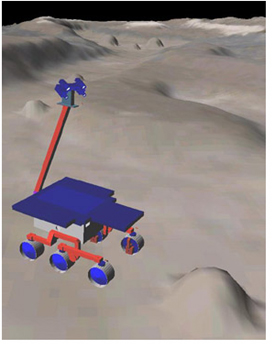
\includegraphics[width=0.5\linewidth]{image/107988main_Sim3.jpg}
    \caption{A rover robot simulated by NASA}
    \label{fig:nasa_robot}
  \end{figure}
  Fourthly, simulation makes it extremely easier to discuss upon, for teaching or demonstrating. By having a virtual model of the robot being your only requirement to show every of its aspects to people, discussing can never be faster and more convenient. If your boss tell you to show what functions have you written for the robot, you can show him visually just by turning your laptop on. If a friend has a great idea for a new way to solve the problem, you can test it immediately.\par
  With its importance, simulation is included in almost every robotic project. Therefore, this document hopefully helps anyone who concerns to find a simple way to make simulations on Linux.
  
  \newpage
  \subsection{Why Linux, ROS and Gazebo?}
  Linux is widely agreed to be the platform for robotics development. This statement is true mostly because of the large amount of supports available in Linux community.\\
  Since the beauty of robotics lies in linking the computer to physical world, Linux infrastructure provides many effective ways to communicate between devices. Most popular hardware and controller, for example Arduino, works very well with Linux. And the processing power of small microcomputers is increasing with a fantastic speed, making portable Linux devices a true thing. That way, the basic functions of robots can be programmed easily on this open-source platform. Moreover, the high quality community with a good knowledge of coding, whose philosophy is to help each other and make a better future with better technology, promote the development of this field dramatically. Therefore, more and more cutting-edge robotic projects are being built on Linux.\\
  Another important property of Linux is that it's free. You don't have to spend thousands of dollars for a software, can make as many robots with operating systems embedded in them as you want, and make experiments without worrying about a "wise investment". For a young university like Vietnamese-German University, I believe Linux is the most suitable researching platform of robotics field.\par
  \begin{figure}[h]
      \centering
      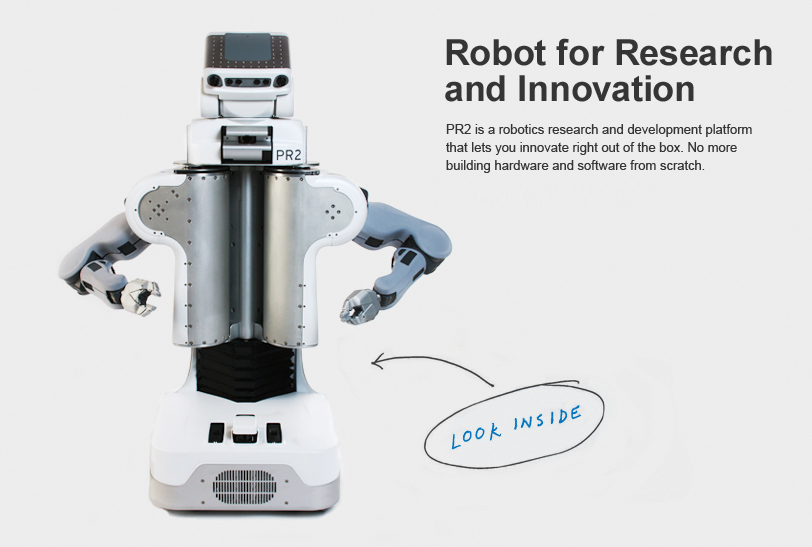
\includegraphics[width=0.8\linewidth]{image/pr2.jpg}
      \caption{PR2 - researching robot running primarily ROS}
      \label{fig:pr2_robot}
  \end{figure}
  However, the most important contributor to that success of Linux in robotics may be ROS. Robotics Operating System, ROS, was created in 2007 by Willow Garage company. Since then, it has unstoppably become one of the most powerful software environment for robotic development.\\
  On contrary to its name, ROS is not really an operating system. It is, in fact, a BSD-licensed open source software framework which runs on Linux. It provides standard  services such as package management, message-passing between processes, low-level device control, and implementation of common functionalities. These service simplifies the basic tasks of a developer, give them more time to concentrate on a specific research idea.\\
  ROS's influence is getting larger and larger. Many researchers and experts contributed to both ROS core ideas and its fundamental software packages, making starting learning robotics a much doable task for beginners like students.\\
  With ROS, a group can freely make their repository publicly available, receiving recognition and credit for their work. This also benefits them with technical feedbacks and improvements like any open-source project. However, they can also start their project on their own server, maintaining full ownership and control over that project. I think this feature is great for a research in a university. Vietnamese-German University can keep all their works on their own server, and publish only what they want.\\
  Therefore, for a newly started robotics department like VGU's, ROS may be the best choice. It's free, easy for students to study, and provide full control over the projects to the university. I personally have started using ROS for a short time, but realized the considerable potential of this platform.\par
  \begin{figure}[h]
      \centering
      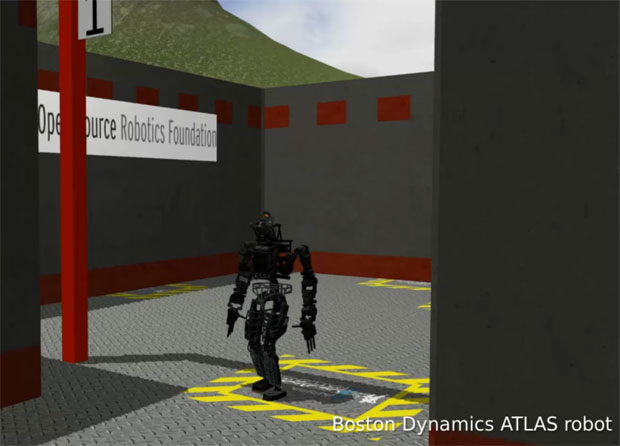
\includegraphics[width=0.65\linewidth]{image/drc_gazebo-1370245661467-1370270174909.jpg}
      \caption{A humanoid robot simulated in Gazebo}
      \label{fig:gazebo_sample}
  \end{figure}
  Lastly, the most important part of this project is the simulator: Gazebo.\\
  Gazebo was founded in 2002 at the University of Southern California. Its original aim was to simulate robots under various conditions in outdoor environment, as the name "gazebo" mean. However, through so many years with improvements, this tool can be used wonderfully in indoor environments.\\
  The highlight of Gazebo is its rich features. It provides accurate and fast simulation in complex environments, thanks to its robust physics engine. It offers advanced 3D graphics, where rendering is so realistic with all high quality textures, shadows and lighting. All kinds of sensors and noise, from contact sensor to Kinect's ones, can be generated optionally. Because of its strong support community, many robot models are available to be downloaded and experiment upon. Gazebo has cloud simulation and also works great with command line tools.\\
  That's why Gazebo has been one of the primary tools for ROS. It is compatible and works great with ROS. What is even better is a great community who support Gazebo, who also work with ROS. Tutorials are available with great details, and questions are answered enthusiastically.\\
  Although Gazebo also runs on Windows and Mac, Linux has always been the focus of its strategies.Therefore, if someone is about to start developing robotics with Linux and ROS, Gazebo is an essential tool to complete the combination.\par
  With all those reasons, Linux, along with ROS and Gazebo, should be choice for robotic researches in a new university like Vietnamese-German University. It offers a free entrance to the field, without trading off the potential for professional researches. It also provides full ownership and control for us to work off-line or on our server. Furthermore, it has a great community to discuss our problems and improve our solutions. In short, it's a perfectly safe and free set of platforms for our work in VGU.
    
  \newpage
  \section{Development}
  \subsection{ROS basics}
  \subsubsection{Basic parts of ROS}
  
  
  \newpage
  \subsubsection{Publishers and Subscribers}
  
  \newpage
  \subsection{Gazebo Simulation}
  Abstract
  
  \newpage
  \subsection{Control Gazebo by ROS}
  Abstract

  \newpage
  \subsection{Project operating timeline}
  Abstract
  
  \newpage
  \subsection{Model design}
  Abstract
  
  \newpage
  \section{Implementation and result}
  \subsection{Model spawning in Gazebo}
  \subsection{Control by ROS}
  \subsection{A simple task}
    
  \newpage
  \section{Conclusion}
  Abstract
  
  \newpage
  \section{Reference}
  Introduction to Robotics: Mechanics and Control, John J. Craig, third edition
  https://www.sharelatex.com/learn/
  http://www.ros.org/history/
  http://www.linuxuser.co.uk/features/linux-is-the-platform-for-robotics
  \begin{lstlisting}
  // Hello.cpp
  #include javax.swing.JApplet;
  import java.awt.Graphics;
  
  public class Hello extends JApplet {
	  public void paintComponent(Graphics g) {
          g.drawString("Hello, world!", 65, 95);
      }    
  }
  \end{lstlisting}
  
\end{document}